%HW13.tex
%Thirteenth Homework -- Math 221H
% 
%
% Frank Sottile
% 27 November 2023 
%
%%%%%%%%%%%%%%%%%%%%%%%%%%%%%%%%%%%%%%%%%%%%%%%%%%%%%%%%
\documentclass[12pt]{article}
\usepackage{amssymb,amsmath}
\usepackage{graphicx}
\usepackage[usenames,dvipsnames,svgnames,table]{xcolor}
\usepackage{multirow}   % This is for more control over tables
%%%%%%%%%%%%%%%%%%%%%%%%%%%%%%%%  Layout     %%%%%%%%%%%%%%%%%%%%%%%%%%%%%%%%%%%%%%
\usepackage{vmargin}
\setpapersize{USletter}
\setmargrb{1cm}{0.25cm}{1cm}{0.5cm} % --- sets all four margins LTRB

%%%%%%%%%%%%%%%%%%%%%%%%%%%%%%%%%%%%%%%%  Macros  %%%%%%%%%%%%%%%%%%%%%%%%%%%%%%%%%%%%%%%%
\newcommand{\RR}{{\mathbb R}}  % This is the backboard bold symbol for the real numbers.  Note how it is used below
\newcommand{\NN}{{\mathbb N}}  % 
\newcommand{\ZZ}{{\mathbb Z}}  %

\newcommand{\calP}{{\mathcal P}}  %Caligraphic P for power set

\newcommand{\bfa}{{\bf a}}    %Vectors
\newcommand{\bfb}{{\bf b}}    %Vectors
\newcommand{\bfF}{{\bf F}}    %Vectors
\newcommand{\bfG}{{\bf G}}    %Vectors
\newcommand{\bfr}{{\bf r}}    %Vectors
\newcommand{\bfS}{{\bf S}}    %Vectors
\newcommand{\bfi}{{\bf i}}    %Unit Vectors
\newcommand{\bfj}{{\bf j}}    %Unit Vectors
\newcommand{\bfk}{{\bf k}}    %Unit Vectors
\newcommand{\bfn}{{\bf n}}    %Unit Vectors

\newcommand{\sep}{{\ :\ }}     % This is for the : in our notation for building sets.
                               % an acceptable (and common) alternative is \mid  (try it!)
%%%%%%%%%%%%%%%%%%%%%%%%%%%%%%%%%%%%%%%%%%%%%%%%%%%%%%%%%%%%%%%%%%%%%%%%
\begin{document}
\LARGE 
\noindent
{\color{Maroon}Honors Multivariate Calculus \hfill Math 221H Section 201}\vspace{2pt}\\
\large
Thirteenth Homework:\hfill 
Due in recitation: Thursday 30 November 2023\vspace{2pt}

\normalsize
    \vspace{2pt}

%%%%%%%%%%%%%%%%%%%%%%%%%%%%%%%%%%%%%%%%%%%%%%%%%%%%%%%%%%%%%%%%%%%%%%%%%%%%%%%%%%%%%%%%%%%%%%%%%%%%
\begin{enumerate}



%%%%%%%%%%%%%%%%%%%%%%%%%%%%%%%%%%%%%%%%%%%%%%%%%%%%%%%%%%%%%%%%%%%%%%%%%%%%%%%%%%%%%%%%%%%%%%%%%%%%
\item  
  Use Green's Theorem to evaluate $\int_C 2xy dx + x^2 dy$, where $C$ is the cardioid curve defined by
  $r=1-\sin(\theta)$.\vspace{-2pt}
%%%%%%%%%%%%%%%%%%%%%%%%%%%%%%%%%%%%%%%%%%%%%%%%%%%%%%%%%%%%%%%%%%%%%%%%%%%%%%%%%%%%%%%%%%%%%%%%%%%%
   
%%%%%%%%%%%%%%%%%%%%%%%%%%%%%%%%%%%%%%%%%%%%%%%%%%%%%%%%%%%%%%%%%%%%%%%%%%%%%%%%%%%%%%%%%%%%%%%%%%%%
\item
  Evaluate the integral ${\displaystyle \iint_D (3xy -4x^2y)\, dA}$ where $D$ is the unit disc directly and using Green's theorem.
  \vspace{-2pt}
%%%%%%%%%%%%%%%%%%%%%%%%%%%%%%%%%%%%%%%%%%%%%%%%%%%%%%%%%%%%%%%%%%%%%%%%%%%%%%%%%%%%%%%%%%%%%%%%%%%%

%%%%%%%%%%%%%%%%%%%%%%%%%%%%%%%%%%%%%%%%%%%%%%%%%%%%%%%%%%%%%%%%%%%%%%%%%%%%%%%%%%%%%%%%%%%%%%%%%%%%
\item Compute the curl $\nabla\times$ and divergence $\nabla \cdot$ of the following vector fields.

  (a) $\bfF(x,y,z) = \sin x \bfi + \cos x \bfj + z^2 \bfk$.


  (b) $\bfF(x,y,z) = e^{xyz}\bfi + \sin(x-y)\bfj - \tfrac{xy}{2}\bfk$.
\vspace{-2pt}
%%%%%%%%%%%%%%%%%%%%%%%%%%%%%%%%%%%%%%%%%%%%%%%%%%%%%%%%%%%%%%%%%%%%%%%%%%%%%%%%%%%%%%%%%%%%%%%%%%%%
   
%%%%%%%%%%%%%%%%%%%%%%%%%%%%%%%%%%%%%%%%%%%%%%%%%%%%%%%%%%%%%%%%%%%%%%%%%%%%%%%%%%%%%%%%%%%%%%%%%%%%
\item Which of the following vector fields on $\RR^3$ are conservative.

  (a) $\bfF(x,y,z)=z\bfi + 2yz\bfj + (x^2+y^2)\bfk$.
  \qquad
  (b) $\bfF(x,y,z)= x\bfi + e^y\sin z \bfj + e^y \cos z\bfk$.
\vspace{-2pt}
%%%%%%%%%%%%%%%%%%%%%%%%%%%%%%%%%%%%%%%%%%%%%%%%%%%%%%%%%%%%%%%%%%%%%%%%%%%%%%%%%%%%%%%%%%%%%%%%%%%%
   
%%%%%%%%%%%%%%%%%%%%%%%%%%%%%%%%%%%%%%%%%%%%%%%%%%%%%%%%%%%%%%%%%%%%%%%%%%%%%%%%%%%%%%%%%%%%%%%%%%%%
\item Suppose that $\bfF$ and $\bfG$ are vector fields whose components have continuous second partial derivatives.
  Prove the identities.

  (a) $\nabla\cdot(\bfF +\bfG) = \nabla\cdot\bfF + \nabla\cdot\bfG$.

  (b) $\nabla(\bfF\cdot\bfG) = (\bfF\cdot\nabla) \bfG + (\bfG\cdot\nabla) \bfF
  + \bfF\times (\nabla\times\bfG) + \bfG\times (\nabla\times\bfF)$.

  The operator $\nabla\cdot\nabla=\frac{\partial^2}{\partial x^2}+\frac{\partial^2}{\partial z^2}+\frac{\partial^2}{\partial z^2}$
  is called the {\color{blue}{\sl Laplacian}} and often written {\color{blue}$\Delta$}.
\vspace{-2pt}
%%%%%%%%%%%%%%%%%%%%%%%%%%%%%%%%%%%%%%%%%%%%%%%%%%%%%%%%%%%%%%%%%%%%%%%%%%%%%%%%%%%%%%%%%%%%%%%%%%%%
   
%%%%%%%%%%%%%%%%%%%%%%%%%%%%%%%%%%%%%%%%%%%%%%%%%%%%%%%%%%%%%%%%%%%%%%%%%%%%%%%%%%%%%%%%%%%%%%%%%%%%
\item Use the normal form of Green's Theorem to deduce {\sl Green's First identity}:
  \[
  \iint_D f\,\nabla^2 g\; dA\ =\ \oint_C f (\nabla g)\cdot \bfn \, ds\ -\ \iint_D \nabla f \cdot \nabla g\; dA\,.
  \]
  Here, $D\subset{\mathbb R}^2$ is a domain with piecewise smooth positively oriented boundary $C=\partial D$ ($C,D$ satisfy the
  hypotheses of Green's Theorem).
\vspace{-2pt}
%%%%%%%%%%%%%%%%%%%%%%%%%%%%%%%%%%%%%%%%%%%%%%%%%%%%%%%%%%%%%%%%%%%%%%%%%%%%%%%%%%%%%%%%%%%%%%%%%%%%

%\newpage

%%%%%%%%%%%%%%%%%%%%%%%%%%%%%%%%%%%%%%%%%%%%%%%%%%%%%%%%%%%%%%%%%%%%%%%%%%%%%%%%%%%%%%%%%%%%%%%%%%%%
\item Evaluate the surface integrals

  (a) ${\displaystyle \iint_S xz\;dS}$, where $S$ is the triangle with vertices $(1,0,0)$, $(0,2,0)$, $(0,0,3)$.

  (b) ${\displaystyle \iint_S (x^2z+y^2z) \, dS}$, where $S$ is the hemisphere $x^2+y^2+z^2=3$ and $z\geq 0$.
  %
  \[
  \begin{picture}(150,110)(0,-10)  \put(10,-10){\small (b) Hemisphere}
%         \put(0,0){\includegraphics[height=100pt]{volume/Hemisphere.eps}}  \end{picture}
         \put(0,0){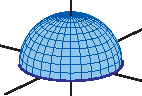
\includegraphics[height=100pt]{images/HW13_1}}  \end{picture}
     \quad 
     \begin{picture}(165,110)(0,-10) \put(10,-10){\small (c) Surface}
%         \put(0,0){\includegraphics[height=100pt]{surface/HypParam.eps}}  \end{picture}
         \put(0,0){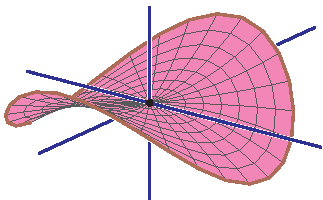
\includegraphics[height=100pt]{images/HW13_2}}  \end{picture}
  \]
  %
  (c) ${\displaystyle\iint_S xy \; dS}$, where $S$ is the surface with parametrization $x=u+v$, $y=u-v$, $z=uv$, and
  $u^2+v^2\leq 1$.\newline
  \mbox{\hspace{35pt}}
  What surface is this?
\vspace{-2pt}
%%%%%%%%%%%%%%%%%%%%%%%%%%%%%%%%%%%%%%%%%%%%%%%%%%%%%%%%%%%%%%%%%%%%%%%%%%%%%%%%%%%%%%%%%%%%%%%%%%%%
   
%%%%%%%%%%%%%%%%%%%%%%%%%%%%%%%%%%%%%%%%%%%%%%%%%%%%%%%%%%%%%%%%%%%%%%%%%%%%%%%%%%%%%%%%%%%%%%%%%%%%
\item Evaluate the surface integral $\iint_S \bfF\cdot \bfn\, dS$, for the given vector field $\bfF$ and surface $S$.

  (a) $\bfF(x,y,z)=xy\bfi - 2 x^2y^2\bfj + yz \bfk$, where $S$ is that part of the paraboloid $z=16-x^2-2y^2$ lying above the
  rectangle $0\leq x\leq 3$ and $0\leq y\leq 2$, oriented upward.

  (b)  $\bfF(x,y,z)= -y\bfi +2x\bfj + 3z \bfk$, where $S$ is the upper hemisphere of the sphere of radius 4, oriented upward.

  (c) $\bfF(x,y,z)= -y\bfi + x\bfj - e^{xz}\bfk$, where $S$ is that part of the cylinder $x^2+y^2=4$ where $1\leq z\leq 4$, and $\bfn$
  is pointing outwards.
  \[
  \begin{picture}(115,110)(0,-10)  \put(10,-10){\small (a) Part of Paraboloid}
%    \put(0,0){\includegraphics[height=100pt]{surface/ParaboloidRectangle.eps}}\ \end{picture}
    \put(0,0){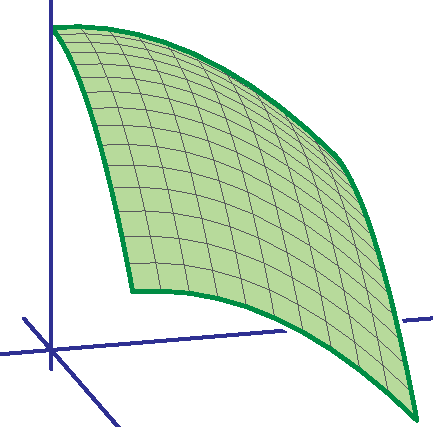
\includegraphics[height=100pt]{images/HW13_3}}\ \end{picture}
  \quad
  \begin{picture}(130,110)(0,-10)  \put(10,-10){\small (b) Hemisphere}
%         \put(0,0){\includegraphics[height=85pt]{volume/Hemisphere.eps}}  \end{picture}
         \put(0,0){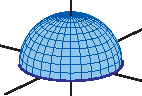
\includegraphics[height=85pt]{images/HW13_1}}  \end{picture}
     \quad 
  \begin{picture}(90,120)(0,-10)  \put(10,-10){\small (c) Cylinder}
%         \put(0,0){\includegraphics[height=115pt]{surface/Cylinder.eps}}  \end{picture}
         \put(0,0){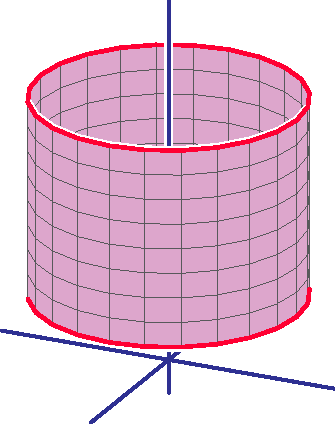
\includegraphics[height=115pt]{images/HW13_4}}  \end{picture}
  \]
 
\vspace{-2pt}
%%%%%%%%%%%%%%%%%%%%%%%%%%%%%%%%%%%%%%%%%%%%%%%%%%%%%%%%%%%%%%%%%%%%%%%%%%%%%%%%%%%%%%%%%%%%%%%%%%%%
   

    
\end{enumerate}



\end{document}
%%%%%%%%%%%%%%%%%%%%%%%%%%%%%%%%%%%%%%%%%%%%%%%%%%%%%%%%%%%%%%%%%%%%%%%%%%%%%%%%%%%%%%%%%%%%%%%%%%%%
\item 
\vspace{-2pt}
%%%%%%%%%%%%%%%%%%%%%%%%%%%%%%%%%%%%%%%%%%%%%%%%%%%%%%%%%%%%%%%%%%%%%%%%%%%%%%%%%%%%%%%%%%%%%%%%%%%%
   

%%%%%%%%%%%%%%%%%%%%%%%%%%%%%%%%%%%%%%%%%%%%%%%%%%%%%%%%%%%%%%%%%%%
polar/Lune

   
%%%%%%%%%%%%%%%%%%%%%%%%%%%%%%%%%%%%%%%%%%%%%%%%%%%%%%%%%%%%%%%%%%%%%%%%%%%%%%%%%%%%%%%%%%%%%%%%%%%%
\item 
\vspace{-2pt}
%%%%%%%%%%%%%%%%%%%%%%%%%%%%%%%%%%%%%%%%%%%%%%%%%%%%%%%%%%%%%%%%%%%%%%%%%%%%%%%%%%%%%%%%%%%%%%%%%%%%
   
